\documentclass[11pt]{article}

\usepackage[T1]{fontenc}
\usepackage[utf8]{inputenc}
\usepackage{lmodern}
\usepackage[margin=0.78in]{geometry}
\usepackage{amsmath,amssymb}
\usepackage{booktabs}
\usepackage{longtable}
\usepackage{tabularx}
\usepackage{array}
\usepackage{enumitem}
\usepackage{xcolor}
\usepackage{graphicx}
\usepackage{microtype}
\usepackage{tikz}
\usepackage{hyperref}
\usepackage{fancyhdr}
\usepackage{caption}

\usetikzlibrary{arrows.meta,calc,fit,positioning,shapes.geometric}

\definecolor{mkblue}{HTML}{246BCE}
\definecolor{mkcyan}{HTML}{168C99}
\definecolor{mkgreen}{HTML}{2D8A52}
\definecolor{mkyellow}{HTML}{D79B18}
\definecolor{mkorange}{HTML}{D66A2C}
\definecolor{mkred}{HTML}{B84040}
\definecolor{mkpurple}{HTML}{7557B7}
\definecolor{mkgray}{HTML}{5E6673}
\definecolor{mklight}{HTML}{F4F7FB}
\definecolor{mkline}{HTML}{CBD4E1}

\hypersetup{
  colorlinks=true,
  linkcolor=mkblue,
  urlcolor=mkblue,
  citecolor=mkgreen,
  pdftitle={MosaicKV Strategy and Failure Analysis},
  pdfauthor={MosaicKV Project}
}

\pagestyle{fancy}
\fancyhf{}
\lhead{MosaicKV Strategy and Failure Analysis}
\rhead{\thepage}
\renewcommand{\headrulewidth}{0.3pt}
\setlength{\headheight}{14pt}

\setlength{\parindent}{0pt}
\setlength{\parskip}{0.52em}
\setlist[itemize]{leftmargin=1.45em,itemsep=0.25em,topsep=0.35em}
\setlist[enumerate]{leftmargin=1.65em,itemsep=0.3em,topsep=0.35em}
\renewcommand{\arraystretch}{1.17}

\newcommand{\code}[1]{\texttt{\detokenize{#1}}}
\newcommand{\artifact}[1]{\path{#1}}
\newcommand{\pass}{\textcolor{mkgreen}{\textbf{PASS}}}
\newcommand{\fail}{\textcolor{mkred}{\textbf{FAIL}}}
\newcommand{\blocked}{\textcolor{mkorange}{\textbf{BLOCKED}}}
\newcommand{\explore}{\textcolor{mkpurple}{\textbf{EXPLORATORY}}}
\newcommand{\negative}{\textcolor{mkred}{\textbf{NEGATIVE}}}
\newcommand{\lesson}{\paragraph{Lesson.}}
\newcommand{\reason}{\paragraph{Why we chose it.}}
\newcommand{\design}{\paragraph{Design and implementation.}}
\newcommand{\experiment}{\paragraph{Experiment.}}
\newcommand{\failure}{\paragraph{Why it failed.}}

\newenvironment{statusbox}[1]{%
  \begin{center}\begin{minipage}{0.95\linewidth}
  \fcolorbox{mkline}{mklight}{\parbox{0.96\linewidth}{\textbf{#1}\par\smallskip}}
  \vspace{0.15em}\small
}{%
  \end{minipage}\end{center}
}

\tikzset{
  stage/.style={draw=mkline, very thick, rounded corners=3pt, fill=white,
    minimum height=9mm, minimum width=22mm, align=center, inner sep=4pt},
  alg/.style={stage, draw=mkblue, fill=mkblue!6},
  data/.style={stage, draw=mkcyan, fill=mkcyan!7},
  good/.style={stage, draw=mkgreen, fill=mkgreen!8},
  bad/.style={stage, draw=mkred, fill=mkred!7},
  warn/.style={stage, draw=mkorange, fill=mkorange!8},
  note/.style={stage, draw=mkpurple, fill=mkpurple!7},
  arrow/.style={-{Latex[length=2.3mm]}, very thick, draw=mkgray},
  failarrow/.style={-{Latex[length=2.3mm]}, very thick, dashed, draw=mkred}
}

\title{\textbf{MosaicKV Strategy and Failure Analysis}\\
\large Designs attempted, experiments performed, failure mechanisms, and lessons learned}
\author{MosaicKV Project}
\date{Evidence cutoff: 17 August 2026\\Repository snapshot: \code{2553f02c6b05b7220ea1a5a691e5f3c15f268c6f}}

\begin{document}

\maketitle

\begin{statusbox}{Scientific-status warning}
This is an engineering and scientific failure-analysis report, not a paper-results section.
It includes clean held-out results, negative calibration outcomes, dirty-worktree exploratory
measurements, implementation failures, and unsupported paths.  Each is labeled separately.
Numbers are copied from inspectable repository documents or immutable run artifacts; no number
is synthetic.  The v85 held-out campaign completed after the first draft of this report.  Its
immutable negative seal and untouched result are now included without retuning the v84 candidate.
\end{statusbox}

\begin{statusbox}{The short conclusion}
MosaicKV repeatedly met the memory goal, often using roughly 34--40\% fewer active key--value
(KV) bytes than Prompt Attention Top-K.  It did \emph{not} yet establish robust end-to-end
superiority.  Early experiments were invalidated by impossible cache geometry, capacity bugs,
or exact-only fallback.  Later experiments were technically valid but failed calibration or
untouched held-out quality.  The strongest completed calibration, v84, passed its memory and
label-blind fidelity gates, but its preregistered v85 held-out validation failed the frozen quality
gate.  Memory and comparison to Prompt Top-K passed; comparison to FullKV did not.
\end{statusbox}

\tableofcontents
\clearpage

\section{Purpose and scope}

Scientific progress is often described only through the final successful method.  That style is
dangerous for MosaicKV because many plausible ideas produced attractive intermediate numbers for
the wrong reason.  Examples include a prototype method that silently ran exact-only, a small
eight-example gate that passed before a larger clean test failed, and a compressed cache whose
active graphics-processing-unit (GPU) bytes fell while its unused central-processing-unit (CPU)
residual tier remained large.  This report preserves the complete causal trail.

The report answers four questions for every major strategy:

\begin{enumerate}
  \item What problem was the strategy meant to solve?
  \item How was it designed and implemented?
  \item What experiment tested it, under what evidence classification?
  \item Why did it fail, or why was its apparent success insufficient?
\end{enumerate}

The primary evidence sources are the versioned Choice-C protocols and seals, the component and
repair ablations, the systems microbenchmark report, and immutable analysis artifacts under
\artifact{/scratch/djy8hg/runs/mosaickv}.  This report includes the completed and sealed v85
held-out outcome.  No v85 answer, reference, score, or failure identity changed the frozen v84
candidate.

\subsection{What ``failure'' means in this report}

Not all failures have the same scientific meaning.  We use the following taxonomy.

\begin{longtable}{>{\bfseries}p{0.19\linewidth}p{0.34\linewidth}p{0.39\linewidth}}
\toprule
Failure class & Meaning & Proper response \\
\midrule
\endhead
Representation infeasibility & The requested compression ratio cannot be represented by the
chosen anchors, prototypes, block size, or per-head layout. & Reject before model execution;
change geometry, not the acceptance threshold. \\
Correctness defect & Code violates the intended algorithm, corrupts ownership, double-frees
storage, miscounts capacity, or silently changes method. & Fix the defect; invalidate affected
claims; rerun on a fresh ledger if outcomes were exposed. \\
Measurement defect & The reported quantity does not match the registered accounting boundary or
timing protocol. & Correct the analyzer or instrumentation; derive again from immutable raw rows
when possible. \\
Calibration failure & No candidate passes a gate using the permitted label-blind calibration
signals. & Freeze nothing; do not evaluate held-out data. \\
Held-out failure & A frozen candidate fails on untouched examples. & Seal the result as negative;
never tune on those labels; start a new version with new calibration data. \\
Systems failure & Quality may be acceptable, but planning, packing, or repair overhead erases
decode savings. & Profile the dominant phase and optimize without changing the algorithmic
contract; report latency even when secondary. \\
Support boundary & An engine or adapter cannot safely express the cache mutation. & Mark the
combination unsupported; do not create simulated native rows. \\
Insufficient evidence & A tiny, dirty, or diagnostic run passes, but cannot support a general or
paper-ready claim. & Treat it as implementation evidence and replicate cleanly on larger,
disjoint data. \\
\bottomrule
\end{longtable}

\section{Research problem and the intended MosaicKV solution}

\subsection{Why multimodal KV caches are difficult}

A vision--language model (VLM) converts a prompt, an image, or a video into a long token sequence.
At every language-model layer and KV head, it stores a key tensor $K$ and value tensor $V$ for
each source position.  During autoregressive decoding, a new query $q_t$ attends to those cached
positions:

\begin{equation}
  \mathrm{Attention}(q_t,K,V)
  = \mathrm{softmax}\!\left(\frac{q_tK^\top}{\sqrt{d}}\right)V.
\end{equation}

The cache grows with the number of visual tokens, layers, and heads.  Simply retaining the largest
prompt attention values is fast, but it can remove a small text region, chart legend, or cross-modal
bridge that matters only during a future decode step.  MosaicKV was designed to preserve such
evidence under a measured byte budget without training the model.

\subsection{The six-component design}

The complete design contains all six mechanisms in Figure~\ref{fig:pipeline}.  Removing one is an
ablation or a reduced variant, not automatically evidence for complete MosaicKV.

\begin{figure}[ht]
\centering
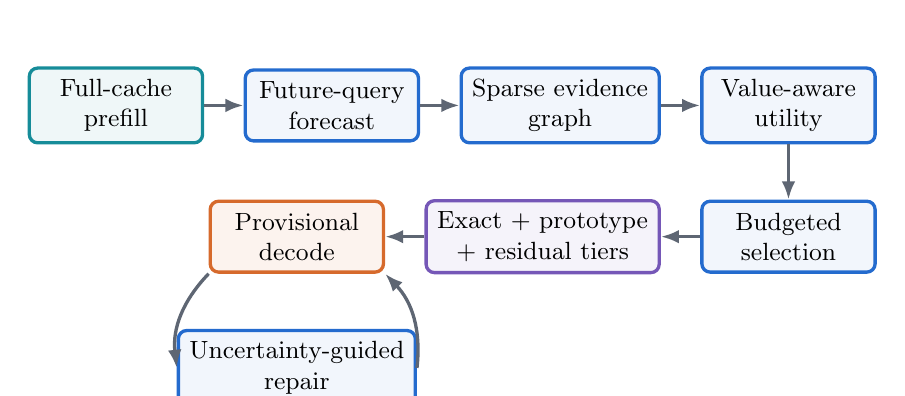
\begin{tikzpicture}[node distance=5mm and 5mm, font=\small]
  \node[data] (full) {Full-cache\\prefill};
  \node[alg, right=of full] (forecast) {Future-query\\forecast};
  \node[alg, right=of forecast] (graph) {Sparse evidence\\graph};
  \node[alg, right=of graph] (utility) {Value-aware\\utility};
  \node[alg, below=7mm of utility] (select) {Budgeted\\selection};
  \node[note, left=of select] (tiers) {Exact + prototype\\+ residual tiers};
  \node[warn, left=of tiers] (decode) {Provisional\\decode};
  \node[alg, below=7mm of decode] (repair) {Uncertainty-guided\\repair};
  \draw[arrow] (full) -- (forecast);
  \draw[arrow] (forecast) -- (graph);
  \draw[arrow] (graph) -- (utility);
  \draw[arrow] (utility) -- (select);
  \draw[arrow] (select) -- (tiers);
  \draw[arrow] (tiers) -- (decode);
  \draw[arrow] (decode.south west) to[bend right=25] (repair.west);
  \draw[arrow] (repair.east) to[bend right=25] (decode.south east);
\end{tikzpicture}
\caption{The intended complete MosaicKV pipeline.  Several experiments in this report exercised
only an exact-selection subset because prototype or repair gates failed.}
\label{fig:pipeline}
\end{figure}

\paragraph{Future-query forecasting.}
The prompt-window mode summarizes recent prompt queries; draft rollout temporarily generates
greedy tokens from the original prefill; hybrid mode combines both.  The goal is to predict what
later queries will need, rather than assuming the last prompt query is sufficient.

\paragraph{Sparse cross-modal evidence graph.}
Each selectable block is a node.  Sparse edges express semantic similarity, attention
co-activation, spatial or layout adjacency, temporal adjacency, common evidence regions, and
cross-modal alignment.  The graph should preserve coverage and diversity without forming an
$O(n^2)$ dense matrix.

\paragraph{Value-aware utility and budgeted selection.}
Forecast attention, expected output contribution, novelty, graph coverage, modality rarity,
redundancy, and mandatory-token priority produce block utility.  Lazy greedy selection chooses
blocks under a hard active-byte budget.

\paragraph{Three cache tiers.}
High-utility blocks remain exact.  Compatible unselected blocks can be summarized by
position-safe prototypes.  Original prototype members can remain in CPU residual storage for
possible restoration.  Active physical length, original logical length, and next decode position
are separate state variables.

\paragraph{Residual repair.}
Entropy and prototype risk can trigger restoration of a bounded number of original residual
blocks.  The current token is then recomputed at most once.  Repair is useful only if it recovers
quality often enough to justify storage and re-decode overhead.

\subsection{The central evaluation gates}

The later campaign compared MosaicKV to Prompt Attention Top-K using measured bytes, not nominal
retention percentages.  If $B_M$ and $B_P$ are mean active KV bytes for MosaicKV and Prompt Top-K,
the registered memory reduction is

\begin{equation}
  R_{\mathrm{active}} = 1 - \frac{B_M}{B_P}.
\end{equation}

The main memory condition is $R_{\mathrm{active}}\ge 0.30$.  When a residual tier exists, the same
30\% condition is also applied to active plus residual bytes in calibration.  This prevents an
apparently small GPU cache from hiding a large CPU cache.

Calibration uses output fidelity without benchmark labels.  Later protocols require the
candidate's FullKV answer agreement to be no more than five percentage points below Prompt Top-K
on every calibration task.  Held-out quality uses paired official task scores.  The registered
gate requires both a nonnegative paired mean difference and a paired-bootstrap lower confidence
bound no worse than the noninferiority margin.  Latency was initially a rejection condition in
early engineering gates, but was later made an informational secondary metric; that policy change
is explicitly recorded rather than applied retroactively.

\section{Chronology at a glance}

Figure~\ref{fig:funnel} shows why a promising implementation result is not automatically a paper
result.  Each stage removes a different kind of false success.

\begin{figure}[ht]
\centering
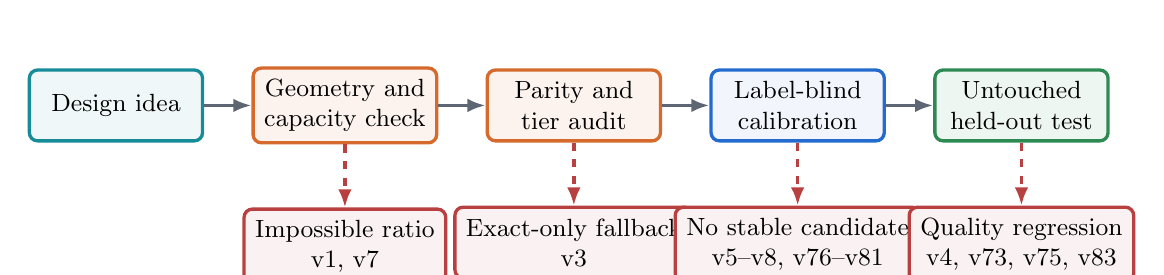
\begin{tikzpicture}[node distance=6mm, font=\small]
  \node[data] (idea) {Design idea};
  \node[warn, right=of idea] (feasible) {Geometry and\\capacity check};
  \node[warn, right=of feasible] (correct) {Parity and\\tier audit};
  \node[alg, right=of correct] (cal) {Label-blind\\calibration};
  \node[good, right=of cal] (held) {Untouched\\held-out test};
  \draw[arrow] (idea)--(feasible);
  \draw[arrow] (feasible)--(correct);
  \draw[arrow] (correct)--(cal);
  \draw[arrow] (cal)--(held);
  \node[bad, below=8mm of feasible] (f1) {Impossible ratio\\v1, v7};
  \node[bad, below=8mm of correct] (f2) {Exact-only fallback\\v3};
  \node[bad, below=8mm of cal] (f3) {No stable candidate\\v5--v8, v76--v81};
  \node[bad, below=8mm of held] (f4) {Quality regression\\v4, v73, v75, v83};
  \draw[failarrow] (feasible)--(f1);
  \draw[failarrow] (correct)--(f2);
  \draw[failarrow] (cal)--(f3);
  \draw[failarrow] (held)--(f4);
\end{tikzpicture}
\caption{The fail-closed scientific funnel.  A failure at one level blocks all later claims.}
\label{fig:funnel}
\end{figure}

\begin{longtable}{p{0.12\linewidth}p{0.24\linewidth}p{0.18\linewidth}p{0.37\linewidth}}
\toprule
Version or study & Main strategy & Outcome & Key reason \\
\midrule
\endhead
Choice C v1 & One exact anchor plus one prototype per three source blocks & \blocked & Minimum
active ratio was $2/3$, so a 0.2 target was mathematically impossible. \\
v2--v3 & Per-head capacity-aware reservations and prototype-cover repair & \blocked / invalid for
full method & Capacity defects were fixed, but v3's apparent 40.74\% advantage was exact-only
fallback, not three-tier MosaicKV. \\
v4 & Genuine exact/prototype/residual held-out path & \negative & Fidelity error was 61.98\% worse
than Prompt Top-K; repair triggered zero times. \\
v5--v6 & Bootstrap-stable label-free profile selection & \negative & Best selection frequencies
were 50.4\% and 52.2\%, below the 60\% gate. \\
v7 & Coordinate-wise consensus profile and exact-head routing & \blocked & Nine full-source exact
head routes could not fit a 20\% dense cache. \\
v8 & Prototype-only sensitive-head routing and repair calibration & \negative & Three-tier routing
worked, but no repair rule met both 10\% trigger and 50\% precision gates. \\
System v70 & Compact routed planner & \negative & Only 12.68\% smaller and 9.82\% slower than Prompt
Top-K; planner preparation was still expensive. \\
System v71 & Lower byte target & \explore & 35.21\% smaller with paired quality on two samples, but
8.03\% slower and too small/dirty for a claim. \\
Quality v72 & Eight examples on three tasks & \explore & Passed a development memory--quality gate,
but the worktree was dirty and the sample was too small. \\
Quality v73 & Clean 48-example replication on three tasks & \negative & MMStar passed; DocVQA and
ChartQA failed quality gates. \\
v74.1--v74.5 & Spatial evidence, byte caps, exact dominance, 8/4-token blocks & \negative & Memory
became feasible, but no candidate met the five-point fidelity gate. \\
v74.6 & Prompt/chart bounded prototypes & \pass\ calibration & Passed 16+16 label-blind calibration;
not a held-out result. \\
v75 & Frozen v74.6 held-out on 48 examples/task & \negative & MMStar and ChartQA passed; DocVQA
failed against both FullKV and Prompt Top-K. \\
v76 & OCR grids and stratified prompt reservations & \negative & Spatial reservations affected
only 32 routed heads while 992 stable heads dominated allocation. \\
v78 & Fixed 50/60\% stable-head visual quota & \negative & Replacing prompt evidence with visual
capacity did not improve worst-task answer agreement. \\
v79 & Adaptive evidence-gain swaps & \negative & Hundreds of swaps caused mixed improvements and
regressions; swap count did not predict output changes. \\
v80 & Per-head future-query risk gate & \negative & It changed too few blocks; the no-swap cache
already contained the main fidelity deficit. \\
v81 & Same-byte prototype decomposition plus prompt-window reranking & \negative & Prototypes gave
no answer advantage; prompt and ``future'' evidence were effectively identical, so zero reranks
were accepted. \\
v82 & Deterministic draft/hybrid forecast with divergence gate & \pass calibration & A frozen
exact-only candidate passed label-blind calibration, but needed untouched validation. \\
v83 & Frozen v82 candidate, 96 examples/task & \negative & Memory passed; both tasks failed strict
paired quality gates despite small mean differences. \\
v84 & Per-swap risk-gated hybrid forecast, 96 examples/task & \pass calibration & Frozen exact-only
candidate passed calibration; it was then evaluated unchanged in v85. \\
v85 & Frozen v84 candidate, 128 examples/task & \negative & Both memory gates and comparison to
Prompt Top-K passed; both tasks failed the required comparison to FullKV. \\
\bottomrule
\end{longtable}

\section{Strategy family I: making the cache representation feasible}

\subsection{Fixed-size blocks and the prototype-geometry failure}

\reason
Fixed-size blocks make the principal budget cardinality-based, keep every block inside one layer
and KV head, and make exact byte accounting predictable.  Prototypes were intended to represent
many discarded blocks with a smaller number of active slots.

\design
The earliest Choice-C geometry used one exact anchor and one prototype for every three source
blocks.  With block size 16 and group size two, each three-block group required at least two active
representatives: one exact block plus one prototype.

\failure
The design had a hard lower bound of $2/3$ active representation.  It could not represent the
requested 0.2 active ratio even with perfect selection.  Revision 1 was cancelled before a result
row completed; partial traces were archived rather than interpreted.  Revision 2 introduced an
analytical feasibility check and increased prototype group sizes to 15 or 31 with matching spans.

\lesson
Compression feasibility must be proven from representation geometry before loading a model.  A
selector cannot compensate for a tier design whose minimum cost exceeds the budget.

\subsection{Per-head dense capacity and reservation ordering}

\reason
Prompt anchors and evidence reservations are useful only if they leave enough per-head capacity
for mandatory blocks and prototype cover.  A global byte total can appear feasible while one
layer/head route is overfull.

\design
The selector added mandatory per-layer/head capacity checks.  Optional partial modality fragments
were excluded in exact mode, and reserved prompt/evidence blocks were allowed to satisfy prototype
anchor coverage.

\failure
Revision 2 rejected three prompt-anchor reservations during calibration.  Revision 3 fixed the
per-head capacity condition but still filled dense capacity with reservations before constructing
the prototype cover.  Consequently every requested \code{mosaickv_full} row used effective method
\code{mosaickv_full__exact_only_incompatible_assignments}.  Its numerical 40.74\% fidelity-error
improvement was invalid as evidence for full MosaicKV because no prototype, residual, or repair
path ran.

Revision 4 moved deterministic prototype coverage into the same budget transaction before bounded
prompt and evidence reservations.  Because the earlier held-out examples had been exposed, v4
used a new ledger rather than recycling them.

\lesson
The effective runtime method must be audited, not inferred from the requested method name.  A good
number from an exact fallback cannot support a three-tier claim.

\subsection{Full-source exact-head routing was incompatible with the budget}

\reason
Per-head routing was introduced to keep stable heads exact and apply costly prototype planning only
to sensitive heads.  This promised better quality and lower planning cost.

\design
Revision 7 used nine full-source exact-head routes chosen from a consensus profile.  Sensitive
heads were routed separately.

\failure
Nine full-source exact routes could not fit inside a 20\% dense Hugging Face (HF) cache.  Every
completed adaptive sample correctly fell back to selection-only.  The job stopped before internal
validation or held-out access.  Revision 8 set \code{exact_head_fraction: 0} and routed sensitive
heads only through smaller, shorter-span prototype groups.

\lesson
``Keep this head exact'' means keeping its entire source sequence, not one cheap scalar decision.
Its byte cost must enter the global transaction before a route is frozen.

\subsection{Block-lattice underfill and padding across heads}

\reason
The later split planner kept 960 stable head routes outside the expensive graph and sent only about
6.25\% of source nodes to the routed planner.  This was the right systems direction, but each head
still needed a length compatible with fixed block granularity and the common packed tensor.

\design
The planner selected the largest feasible block-aligned capacity below a requested per-head length,
used actual selected bytes to update the remaining budget, and inserted padding only when routed
prototype heads and external stable exact heads had different attainable lengths.  Logical
positions remained separate from physical packed positions.

\failure
Early variants demanded exact fill of a 75-position target although 16-token blocks could attain
only 64 positions.  Later variants planned padding for routed heads but not stable external heads,
causing mismatched 75/64 lengths.  These were correctness and accounting defects, not negative
algorithmic results.  Regression tests were added for both cases.

In v70, the split planner reduced roughly 40,000 source nodes to 2,496--2,560 planner nodes and
graph construction averaged 0.146 seconds, but planner preparation still averaged 0.367 seconds.
Stable routes underfilled by 10,560 positions and the final cache was only 12.68\% smaller than
Prompt Top-K.  V71 lowered the target, reached 35.21\% active-memory reduction, and reduced stable
shortfall to 4,800 positions, but planner preparation still averaged 0.460 seconds.

\lesson
Budget feasibility is a lattice problem, not continuous arithmetic.  Configured cap, dense
attainable cap, logical active bytes, padding bytes, final packed bytes, and unavoidable shortfall
must be reported separately.

\section{Strategy family II: choosing a stable configuration without labels}

\subsection{Prompt anchors and a composite FullKV fidelity objective}

\reason
An evidence-heavy utility can evict the question or instruction text.  Prompt anchors reserve a
small part of capacity before graph-based optimization.  Benchmark labels were deliberately
excluded so calibration would not fit DocVQA or ChartQA answers.

\design
The early composite loss was

\begin{equation}
 E=(1-A_{\mathrm{token}})+\log(1+D_{\mathrm{KL}})+E_{\mathrm{attn\mbox{-}out}},
\end{equation}

where $A_{\mathrm{token}}$ is token agreement with FullKV, $D_{\mathrm{KL}}$ is logit Kullback--Leibler
divergence, and $E_{\mathrm{attn\mbox{-}out}}$ is attention-output error.  A robust candidate also
included a 90th-percentile loss term.  Bootstrap resampling estimated whether one profile was a
stable winner.

\experiment
Revision 5 evaluated 20 design examples and 60 candidate rows.  The best profile won 50.4\% of
1,000 bootstrap resamples, below the frozen 60\% threshold.  Revision 6 doubled design examples to
40, fixed a bootstrap eligibility bug, and reran the same selection problem.

\failure
The largest v6 selection frequency was 52.2\%.  The two best profiles differed in mean calibration
loss by only 0.00075.  More samples did not reveal a unique, stable winner because the candidates
were practically tied.  The threshold was not weakened.

\lesson
A low point estimate is not enough.  If the winner changes under ordinary resampling, freezing it
would turn calibration noise into a design choice.

\subsection{Coordinate-wise consensus}

\reason
Because no candidate was a stable winner, revision 7 took the coordinate-wise median of the three
predefined profiles.  This rule did not inspect task labels or candidate rank.

\design
The consensus used utility weights $-0.30/-0.30$, prompt and evidence reservations of 0.15, a
head-shift threshold of 0.15, and prototype geometry of at most 15 blocks or 255 positions.

\failure
The first coordinator exposed an optional partial-fragment reservation bug; after that fix, the
full-source exact-head routing was found infeasible.  Thus consensus solved statistical
instability but not representation capacity.

\lesson
Statistical stability and systems feasibility are independent gates.  A deterministic compromise
can still be impossible to pack.

\section{Strategy family III: forecasting future queries}

\subsection{Prompt-window forecasting}

\reason
Recent prompt queries are already available after prefill and are cheap to summarize.  They are a
natural first estimate of what the decoder will attend to.

\design
For each layer and KV head, the implementation forms prompt means, variances or covariances, and
normalized centroids from the last $w$ prompt positions.  A low-memory path stages one layer of
query samples at a time.

\experiment
The small component ablation used Qwen2.5-VL-3B, two examples per image task and one video example.
Relative to no forecasting, selected-block recall improved by 0.2055 for prompt-only and 0.2888 for
the full hybrid forecast.

\failure
Recall did not consistently become task quality.  Full hybrid minus no-forecast task-score changes
were 0.0000 on MMStar, +0.2353 on DocVQA, $-0.5000$ on ChartQA, and 0.0000 on Video-MME.  The run was
tiny and dirty, so it could guide implementation but not support a quality claim.

\lesson
Oracle-set recall is a diagnostic, not the final objective.  It can reward blocks that resemble
future attention without preserving the exact evidence needed for a discrete answer.

\subsection{Draft and hybrid forecasting}

\reason
A temporary greedy draft observes query vectors that do not exist in the prompt.  It reuses the
original prefill, clones cache state, performs a bounded rollout, and discards the draft tokens.
Hybrid mode combines this genuinely future-facing evidence with stable prompt statistics.

\design
Per-head routing lets stable heads trust prompt queries and shifted heads trust draft queries.
Later exact-only candidates reranked stable-head blocks when draft/prompt distributions diverged.
A total-variation gate failed closed if the alleged future distribution was indistinguishable from
the prompt distribution.

\failure
Prompt-only reranking (v81) compared a prototype cache, an equal-byte exact-only cache, and exact
cache variants reranked by a prompt-window ``future'' signal.
Each sample exposed about 11,904 rerank candidates, but zero
reranks were accepted.  The prompt-derived forecast reused the same evidence that produced Prompt
Top-K, so the ranking signal did not diverge.  All candidates failed fidelity despite 34.55\%
memory reduction.

\paragraph{Partial success, then held-out failure (v82--v83).}
V82 added deterministic two- and four-token draft rollouts, hybrid forecasts, and an explicit
divergence gate.  On 64 disjoint calibration examples per task, the selected four-draft exact
candidate reduced active bytes by 35.14\% on DocVQA and 34.47\% on TextVQA.  Its FullKV answer
agreement exceeded Prompt Top-K by 4.6875 and 3.125 percentage points, respectively.  This was a
valid positive calibration and produced a frozen candidate.

V83 evaluated that frozen candidate once on 96 untouched examples per task.  Memory still passed:
34.86\% lower active bytes on DocVQA and 34.85\% on TextVQA.  Quality did not.  Table~\ref{tab:v83}
shows the exact paired outcomes.

\begin{table}[ht]
\centering
\small
\caption{V83 clean held-out result for the frozen v82 exact-only hybrid candidate.}
\label{tab:v83}
\begin{tabular}{lrrrrl}
\toprule
Task & $N$ & Active reduction & $\Delta$ vs FullKV & 95\% paired CI & Gate \\
\midrule
DocVQA & 96 & 34.86\% & $-0.00017$ & [$-0.01501$, 0.01609] & \fail \\
TextVQA & 96 & 34.85\% & $-0.02083$ & [$-0.05208$, 0.00000] & \fail \\
\bottomrule
\end{tabular}
\end{table}

The candidate also had negative mean score differences versus Prompt Top-K: $-0.01280$ on DocVQA
and $-0.00417$ on TextVQA.  The strict preregistration required a nonnegative mean, so even the
nearly zero DocVQA difference failed.  The TextVQA lower confidence bound against FullKV also fell
slightly beyond the $-0.05$ noninferiority margin.  Median end-to-end latency was 15.65\% and
15.87\% higher than Prompt Top-K; latency was informational and did not cause rejection.

\lesson
Draft queries created a real and useful ranking difference, but calibration success did not
generalize reliably.  A positive disjoint calibration is a reason to run held-out validation, not
a result to publish as superiority.

\subsection{Per-swap forecast-risk gating (v84)}

\reason
Broad reranking can replace a safe prompt block with a speculative future block.  V84 scored each
proposed swap and accepted it only when forecast gain justified prompt-mass loss; moderate and
conservative risk gates were compared to a no-rerank control.

\design
The method used a four-token hybrid forecast, four-token blocks, a 27.5 MB configured cap, exact
tiers only, and zero residual storage.  Every sample needed at least one route whose prompt and
forecast distributions diverged.  A risk-gated arm needed both accepted and rejected swaps on
every task and could not underperform the no-rerank control in FullKV answer agreement.

\experiment
On 96 fresh calibration examples per task, the moderate candidate reduced active bytes by 34.68\%
on DocVQA and 34.44\% on TextVQA.  It exceeded Prompt Top-K FullKV answer agreement by 3.125
percentage points on both tasks.  It accepted about 404.5 swaps per DocVQA sample and 333.6 per
TextVQA sample while risk-rejecting about 5,952.6 and 5,727.6.

\paragraph{Why calibration was not success.}
V84 is a positive calibration result, not an untouched evaluation.  Its token agreement with
FullKV remained low (0.2692 DocVQA and 0.2446 TextVQA), showing that exact answer agreement can hide
large sequence differences.  The frozen candidate therefore required v85 held-out validation.

\subsection{Frozen v85 held-out result}

V85 ran the unchanged v84 candidate on 128 new DocVQA and 128 new TextVQA examples.  It completed
1,536 measured rows with zero failed rows, missing required values, nonfinite timings, residual
bytes, or repairs.  Every method was deterministic across two repetitions.  The protocol label was
\code{mosaickv_full}, but the trace and analyzer correctly reported the effective method as
\code{mosaickv_exact}, tier mode \code{exact_only_prototypes_disabled}.  V85 therefore cannot
support prototype, residual-repair, or complete six-component MosaicKV claims.

The active and active-plus-residual memory gates passed on both tasks.  MosaicKV used 26,529,792
bytes on DocVQA and 26,411,008 bytes on TextVQA, respectively 34.85\% and 34.89\% below Prompt
Top-K.  Residual bytes were exactly zero, so active and total-memory reductions were identical.

Quality against Prompt Top-K passed.  MosaicKV improved mean score by 0.02123 on DocVQA with a
95\% paired-bootstrap interval of [$-0.00444$, 0.05113], and by 0.02031 on TextVQA with interval
[$-0.00781$, 0.05469].  The required FullKV comparison failed.  DocVQA's difference was
$-0.00513$ with interval [$-0.03495$, 0.02599]: its noninferiority interval passed, but the frozen
nonnegative-mean rule did not.  TextVQA's difference was $-0.04609$ with interval
[$-0.09219$,$-0.00703$], failing both the nonnegative-mean rule and the $-0.05$ noninferiority
lower bound.

Latency remained informational.  The paired median MosaicKV/Prompt-Top-K end-to-end ratios were
1.1747 on DocVQA and 1.1789 on TextVQA.  Decode p50 was slightly lower for MosaicKV, but its
4.21/4.13-second compression p50 exceeded Prompt Top-K's 3.05/3.02 seconds and dominated the
end-to-end difference.  The immutable result is sealed in
\artifact{mosaickv/configs/ledgers/choice_c_v85_negative_heldout_seal.yaml}.

\section{Strategy family IV: evidence graphs and modality preservation}

\subsection{Sparse cross-modal graph}

\reason
Prompt attention alone ranks blocks independently.  Documents and charts often require a group:
a question word, a text region, its nearby value, and a spatial relationship.  Facility-location
coverage over a graph was intended to keep representative evidence clusters.

\design
The graph pooled key, value, and optional hidden-state descriptors; added compatible semantic,
attention co-activation, spatial/layout, temporal, same-region, and cross-modal edges; and kept
only top-$d$ neighbors.  Chunked top-$k$ construction avoided a dense $n\times n$ matrix.  A
degree-four graph replaced degree eight after the latter diffused coverage on design data.

\experiment
In the bounded component ablation, removing the graph reduced facility coverage by 0.8326 on the
structured DocVQA/ChartQA subset and 0.8114 on MMStar.  Yet full-minus-no-graph task-score changes
were zero on MMStar, DocVQA, ChartQA, and Video-MME.  The graph improved attention-output error by
0.0008 on structured tasks but worsened it by 0.0651 on MMStar.

\failure
The available task records exposed processor visual-grid boxes and frame indices, but not
benchmark OCR strings, table cells, or named layout regions.  Consequently many intended edges
were generic geometric or semantic proxies.  Increased facility coverage showed the graph was
doing what its objective requested, but not that the covered clusters contained answer-critical
evidence.

\lesson
Coverage is only meaningful when edge semantics match the task's evidence structure.  More graph
coverage can be a better solution to the wrong graph.

\subsection{V74 spatial evidence and byte-cap sequence}

\reason
After v73 failed on DocVQA and ChartQA, the next hypothesis was that routed selection lacked
spatial/OCR evidence.  V74 tested spatial anchors, evidence reservations, bounded prototypes,
exact-dominant variants, finer blocks, and precise byte caps without using benchmark labels.

\design and outcomes
The sequence is important because each revision fixed a different confound:

\begin{itemize}
  \item \textbf{v74.1:} spatial candidates used only 26.44\% less active-plus-residual memory than
  Prompt Top-K, so every candidate was memory-ineligible regardless of answer agreement.
  \item \textbf{v74.2:} 32--35 MB byte caps achieved 43.99--48.11\% reductions, but worst-task
  FullKV answer agreement was only 31.25--37.50\%; all failed fidelity.
  \item \textbf{v74.3:} explicit configured, attainable, planner, logical, padding, and packed-byte
  telemetry removed a double-cap ambiguity.  Exact-dominant 27.5--29 MB candidates achieved
  36.30--36.56\% reductions, but worst agreement remained 43.75--50.00\%.
  \item \textbf{v74.4:} common eight-token blocks improved worst agreement to 62.50--68.75\% while
  retaining 31.63--34.55\% reduction, but no arm met the five-point fidelity gate.
  \item \textbf{v74.5:} common four-token blocks eliminated stable-head shortfall and padding
  underfill, but worst agreement fell to 50.00--56.25\%.  Finer granularity increased choice; it
  did not guarantee that the utility chose the right evidence.
  \item \textbf{v74.6:} one-pass bounded prototype planning finally honored a one- or two-prototype
  limit.  The chart-oriented candidate used 64 prototypes, retained about 92.37\% exact prompt
  mass and 93.48\% represented prompt mass, reduced total measured memory by 35.29\%, and matched
  Prompt Top-K FullKV answer agreement on 16 DocVQA and 16 ChartQA calibration examples.  It was
  frozen for v75.
\end{itemize}

\failure
V75 tested the frozen v74.6 candidate on 48 examples each from DocVQA, MMStar, and ChartQA.  Memory
passed on all tasks.  MMStar and ChartQA quality passed; DocVQA did not.  Against FullKV, DocVQA's
mean score difference was $-0.04097$ with a 95\% paired interval of
[$-0.10069$, 0.00139].  Against Prompt Top-K it was $-0.00759$ with interval
[$-0.03125$, 0.00570].  Answer agreement was 58.33\% with FullKV and 75\% with Prompt Top-K.

\lesson
Spatial/chart-oriented calibration transferred to ChartQA and a general task but not reliably to
documents.  Aggregate prompt mass near 93\% was misleading because text dominated prompt
attention; it did not prove that small visual OCR regions survived.

\subsection{OCR grids and prompt stratification (v76)}

\reason
V76 attempted to reserve more uniformly distributed image evidence with four- and six-cell OCR
grids while maintaining prompt-stratified exact capacity.

\design
The change applied to 32 routed heads.  The other 992 stable heads continued to use exact Prompt
Top-K selection.  The byte cap, four-token blocks, memory gate, and five-point fidelity gate were
unchanged on 16 DocVQA and 16 TextVQA calibration examples.

\failure
All candidates achieved 34.74\% total reduction but failed fidelity.  The v74 control and six-grid
candidate had only 43.75\% worst-task FullKV answer agreement; the four-grid candidate had 37.50\%.
The audit explained why: image tokens carried only about 10.96\% of prompt mass.  Stable-head text
retention was already about 99.74\%, and spatial reservations on 32 routed heads barely changed
the global image allocation.  Prompt Top-K retained 44.38\% of image exact mass on DocVQA versus
roughly 33\% for the v76 candidates.

\lesson
A mechanism applied to 3.125\% of heads cannot repair a global modality imbalance controlled by
the other 96.875\%.

\subsection{Fixed visual quotas (v78)}

\reason
To affect stable heads directly, v78 forced 50\% or 60\% visual capacity before ranking within
visual and text groups.

\failure
All arms reduced memory by 34.20\% but failed fidelity.  Worst-task answer agreement remained
62.50\%.  The 50\% and 60\% quotas lowered exact prompt mass from 92.78\% to 91.87\% and 90.63\%,
and macro token agreement fell from 27.98\% to 26.27\% and 18.85\%.  Uniform quotas replaced useful
text blocks even on heads where visual evidence did not justify the exchange.

\lesson
Modality balance should be evidence-adaptive and head-specific, not an unconditional percentage.

\subsection{Adaptive stable-head swaps (v79)}

\reason
V79 allowed a visual block to replace a text block only when evidence gain exceeded prompt-mass
loss and a minimum text-mass fraction remained.

\design
Two policies were tested: a conservative 99.75\% text-preservation/1.50 gain rule and a broader
99.5\%/1.25 rule.  The total bytes were unchanged, so any result isolated selection quality.

\failure
On 32 examples per task, all arms passed 34.80\% memory reduction but failed fidelity.  The
conservative rule made about 365.5 swaps per DocVQA sample and 319.4 per TextVQA sample; the broad
rule made about 754.4 and 689.4.  Improvements and regressions were balanced or worse.  Correlation
between aggregate swap count and answer change was $-0.1576$ to $-0.0018$, providing no useful
causal signal.  Compact traces also omitted exact per-head accepted pairs, so stronger attribution
would have been speculation.

\lesson
Aggregate activity is not causal evidence.  Per-head accepted/rejected pairs must be recorded, and
the selection policy must distinguish high-risk token-decision swaps from harmless ones.

\subsection{Per-head risk-gated swaps (v80)}

\reason
V80 added future-query gain, prompt-loss limits, and per-head risk records so only low-risk swaps
would occur.

\failure
On 48 examples per task, strict and balanced gates produced almost the same metrics as the no-swap
control: about 34.41\% memory reduction, 62.50\% worst-task answer agreement, and 25.42--25.47\%
macro token agreement.  The gate changed too few selected blocks to repair quality.  More
importantly, the no-swap prototype cache already contained the dominant fidelity gap.  Tuning the
swap guard could not fix an error created earlier by prototype/exact decomposition.

\lesson
Optimize the stage that causes the error.  A careful late-stage gate cannot recover evidence that
the underlying representation already distorted.

\section{Strategy family V: value-aware utility and submodular selection}

\subsection{Why value information was added}

Prompt attention estimates where the prompt looked, but values determine the vector returned by
attention.  MosaicKV therefore included expected output contribution and novelty relative to
neighbors, then used facility-location and modality coverage to discourage redundant selections.

The registered local utility used signed coefficients so contribution and uniqueness became
preservation rewards rather than accidental eviction penalties.  Lazy greedy selection cached
marginal gains and used deterministic tie-breaking.

\subsection{What the ablation showed}

In the current small component ablation, removing value contribution increased mean
attention-output error by 0.0023, which favors the value-aware full configuration.  However, it
changed mean logit KL by $-0.0085$, which favors the ablation.  Earlier diagnostics had shown the
opposite mix before the sign correction.  Thus value information affected internal fidelity, but
not consistently across metrics.

\failure
The utility optimized continuous proxies whose relationship to discrete answer quality varied by
task and model.  A small change in attention-output error need not cross a greedy token decision
boundary; conversely, a near-tied logit can flip with a tiny numeric change.  Monotonicity and
diminishing-return unit tests validate the selector mathematics under its assumptions, not the
assumption that its features identify answer-critical evidence.

\lesson
Utility quality must be evaluated by paired future-token decisions and task outcomes as well as
attention reconstruction.  No single surrogate was consistently sufficient.

\section{Strategy family VI: RoPE-safe prototypes}

\subsection{Why ordinary averaging is invalid}

Many adapters cache keys after rotary position embedding (RoPE).  If two keys at different logical
positions are averaged directly, their coordinate systems have different rotations.  The result
is not a meaningful representative key.

\design
The audited HF path neutralizes each member to a common rotary frame, gathers members in original
order, computes weighted key and value means in FP32, chooses a forecast-weighted member-medoid
anchor, and re-applies the anchor phase.  Qwen2.5-VL uses multimodal RoPE coordinates, so temporal,
height, and width phases must all be preserved.  Unsupported adapters fail closed to exact-only.

\subsection{Early safety fallback and later genuine prototypes}

Early component experiments correctly disabled prototypes for post-RoPE Qwen caches because a safe
transform had not yet passed.  Those rows could validate exact selection only.  Later v17
ablations recorded the audited de-rotate/merge/re-rotate transform and labeled 44 three-tier
cells, allowing prototype diagnostics to be interpreted.

\subsection{Why prototypes still failed to establish robust quality}

In the small v17 ablation, prototypes improved attention-output error by 1.0041 and logit KL by
2.9782 relative to exact-only at the same active memory, but task scores were unchanged on the
one- or two-example task subsets.  In v81's larger same-byte decomposition, 64 prototypes gave
exactly zero answer-agreement advantage over exact-only.  They improved token agreement only by
about 0.0093 on DocVQA and 0.0049 on TextVQA.  Removing them also removed residual bytes without an
answer penalty.

\failure
Phase-safe averaging prevents a mathematically invalid key, but it does not make heterogeneous
evidence compressible into one vector.  A prototype can preserve average attention behavior while
erasing the rare word, number, or chart value that decides an answer.  Moreover, residual storage
counts against total memory unless repair supplies a measured quality benefit.

\lesson
RoPE safety is necessary, not sufficient.  Prototype membership must be semantically coherent,
and its quality advantage must beat an exact-only same-byte control on disjoint data.

\section{Strategy family VII: uncertainty-guided residual repair}

\subsection{Original repair policy}

\reason
Compression errors are not equally dangerous.  A low-confidence token or a high-attention,
high-dispersion prototype is a plausible sign that discarded details matter.  Repair aimed to pay
extra latency only on such steps.

\design
For provisional next-token probabilities $p$, normalized entropy is

\begin{equation}
 H_{\mathrm{norm}}=-\frac{\sum_v p_v\log p_v}{\log |\mathcal{V}|}.
\end{equation}

For prototype $j$,

\begin{equation}
 \mathrm{risk}_j=a_j\,\frac{D^{K}_j+D^{V}_j}{2},
\end{equation}

where $a_j$ is its current attention mass and $D^K_j,D^V_j$ are key/value dispersions.  Policies
included none, entropy, prototype risk, their union, and evaluation-only oracle repair.  A trigger
ranked prototype clusters by risk, restored at most $R$ residual blocks from CPU memory, evicted a
low-utility prototype if necessary, and recomputed the current step once.

\subsection{Revision-8 repair calibration failure}

Revision 8 produced genuine three-tier rows and improved registered mean fidelity error from
2.375571 to 2.329087 at equal active bytes; exact selection was much worse at 5.198446.  The oracle
recorded 102 repair triggers, 29 token changes, and 15 FullKV-token recoveries.  Nevertheless, no
online rule met both the frozen 10\% trigger-rate ceiling and 50\% precision floor.  The fail-closed
profile disabled repair and the downstream sweep was blocked.

\subsection{Experiment-4 policy sweep}

The exploratory A100 sweep used seven fixed examples and 105 paired sample-policy rows.  Only one
no-repair answer differed from FullKV and was oracle-repairable.  Table~\ref{tab:repair} preserves
the positive and harmful outcomes.

\begin{table}[ht]
\centering
\small
\caption{Primary residual-repair results from the seven-example exploratory sweep.}
\label{tab:repair}
\begin{tabular}{lrrrrr}
\toprule
Policy & Triggered samples & Precision & Recall & Avg repair ms & E2E cost (s) \\
\midrule
No repair & 0/7 & N/A & 0.0000 & N/A & 0.000 \\
Entropy & 7/7 & 0.1429 & 1.0000 & 505.533 & 10.782 \\
Prototype risk & 5/7 & 0.0000 & 0.0000 & 329.725 & 5.306 \\
Combined risk & 7/7 & 0.0000 & 0.0000 & 418.474 & 13.220 \\
Oracle, evaluation only & 3/7 & 0.3333 & 1.0000 & 381.367 & 0.569 \\
\bottomrule
\end{tabular}
\end{table}

Entropy and oracle repair improved the ChartQA failure.  The original combined policy changed it
to a different wrong number.  A conservative combined threshold repaired that chart but also
changed a DocVQA answer incorrectly, cancelling net quality gain.

\subsection{Targeted repair fixes and their limit}

The repair implementation was improved in three ways: partial prototype promotion subtracted only
restored members and retained remaining members; source blocks were ranked by reconstruction error;
and prototype risk was gated by minimum entropy.  On the same seven examples, guarded prototype
risk repaired the sole compressed failure, raised score sum from 4/7 to 5/7, introduced no wrong
answer changes, and reduced events from 38 to 16.  It still added 3.983 seconds mean end-to-end
latency.

FP8 and INT8 residuals halved mean residual storage from about 53.60 MiB to 26.80 MiB but did not
improve latency.  Each event restored only about 13.4 KiB; re-decode and dequantization, not host
transfer volume, dominated.  $R=1$, $R=2$, and $R=4$ all repaired the same single failure, so larger
$R$ transferred more bytes without a measured quality benefit.

\failure
The trigger problem was severely imbalanced: true repairable failures were rare, but entropy and
risk fired broadly.  Even correct restoration must pay for a synchronized re-decode.  A tiny
seven-example success after targeted changes is useful implementation evidence but cannot estimate
population precision or recall.

\lesson
Repair is justified only when a disjoint calibration set establishes a precise trigger and a
held-out set establishes net quality benefit.  Smaller residual dtype and larger $R$ solve storage
capacity, not trigger precision or re-decode cost.

\section{Strategy family VIII: systems and latency optimization}

\subsection{Why memory reduction did not automatically reduce latency}

Reducing active KV bytes shrinks attention's key/value work, but a decode step still executes model
weights, projections, multilayer perceptrons, Python control, and synchronization.  At batch one
and one-token queries, these fixed costs can dominate.  MosaicKV additionally pays for forecasting,
graph construction, utility, tier construction, cache packing, and possible repair.

An exploratory held-out implementation reported mean component times of 1.3459 seconds for
forecasting, 6.7814 for graph construction, 1.8824 for utility/selection, 13.3481 for tier
construction, and 2.9641 for packing.  Total compression was 26.3218 seconds versus 2.0502 for
Prompt Top-K.  The worktree was dirty, so these numbers diagnose engineering cost rather than
support a paper result.

\subsection{Optimizations attempted}

The implementation added vectorized layer-wise gathering, ordered FP32 prototype reduction,
batched rotary neutralization/rephasing, cached membership sets, sparse stable top-$k$, staged
query transfer, preallocated append-only decode cache, geometric mask/position buffers,
\code{logits_to_keep=1}, no-mask dense exact decoding, and an explicit eager-prefill/SDPA-decode
path.

On a 16-sample parity set, these changes preserved selected blocks and generated tokens while
reducing tier construction from 31.0880 to 13.3570 seconds, graph time from 7.7182 to 6.7596, and
total evaluation-path time from 55.8292 to 37.5283 seconds (32.78\%).  This was a substantial
implementation improvement, but not enough to beat the much simpler baseline.

\subsection{Decode fast path versus compression overhead}

Matched Qwen2.5-VL-3B runs showed that preallocated cache growth lowered FullKV decode by 2.1\% and
MosaicKV exact decode by 1.4\%.  At equal 1,769,472 active bytes, MosaicKV exact decoded in 3.338
seconds versus 3.396 seconds for Prompt Top-K, a 1.7\% decode improvement.  Its 0.778-second
planning cost still made end-to-end latency worse.

The eager-prefill/SDPA-decode path reduced a retention-0.1 exact point from 3.346 to 2.995 seconds
decode and 4.762 to 4.400 seconds end-to-end relative to eager.  Retention-1 parity passed.  This
showed that fused decode helps both methods, not that MosaicKV alone wins; fairness requires the
same backend configuration for every compared row.

In the 440-row systems study, compression overhead outweighed decode savings in all ten listed
Qwen-3B/7B regimes.  LLaVA's vectorized-gather fix made bounded runs finish, but at output length 64
its exact cache decoded at 43.075 ms per token versus FullKV's 42.897 ms.  The regime was
weight/launch-bound, so lower cache bytes did not reduce token latency.

\subsection{Changing the latency gate}

Early engineering gates demanded both 30\% less active memory and 5\% lower end-to-end latency.
V70 was 12.68\% smaller and 9.82\% slower; v71 was 35.21\% smaller and 8.03\% slower.  The research
priority was later changed to require 30\% lower active memory with paired quality noninferiority,
while latency became a reported secondary metric.  This change was prospective.  It did not turn
old latency failures into victories or permit latency to be omitted.

\lesson
MosaicKV's current value proposition is memory--quality, not proven latency.  A paper must report
where compression overhead outweighs decode savings and avoid claiming that byte reduction implies
speedup.

\section{Strategy family IX: native vLLM and SGLang integration}

\subsection{Why native cache mutation was attempted}

HF provides tensor access but not continuous batching.  vLLM and SGLang can improve throughput,
yet their schedulers own physical blocks, logical token counts, request state, and prefix caches.
Dropping a physical block without an atomic metadata transaction can renumber rotary positions,
leak a request's cache, or double-free memory.

\subsection{vLLM transport path}

The version-pinned vLLM 0.10.2 plugin intercepts the complete-prefill scheduler boundary, releases
unselected request-owned blocks, installs null placeholders, sends a replacement table to the
worker, preserves \code{num_computed_tokens}, and filters null blocks during release.  It rejects
prefix caching, CUDA graphs, speculative decoding, multiple cache groups, and unsupported metadata.

Exploratory A100 job 17869843 passed retention-1 token parity, reduced 18 source blocks to nine at
retention 0.5, reduced active storage from 11,132,928 to 5,824,512 bytes, generated valid tokens,
and passed an A--B--A request-isolation probe.

\failure boundary
The selector was only deterministic mandatory/even coverage, not the common MosaicKV
forecast/graph/utility plan.  vLLM exposes no public atomic transaction API equivalent to the
internal patch.  Prototype injection and residual repair remain unsupported.  Therefore the result
is a transport gate, not a native \code{mosaickv_exact} paper row.

\subsection{SGLang transport path and two instructive failures}

The SGLang 0.5.1.post3 patch compacts \code{ReqToTokenPool} ownership, frees dropped token slots,
separates active \code{seq_lens} from logical \code{orig_seq_lens}, preserves Qwen multimodal RoPE
positions, and rejects Radix caching, overlap, graphs, speculation, and recomputation.

Two attempts failed before the final transport gate:

\begin{itemize}
  \item Job 17869844 showed that a patch installed in the parent process does not cross SGLang's
  multiprocessing \code{spawn} boundary.  The engine target had to install the patch inside the
  child before constructing the scheduler.
  \item Job 17870743 showed that disabling Radix selects \code{ChunkCache}; ordinary release then
  tried to free already compacted/zeroed logical slots a second time.  The final path releases only
  compact active ownership and checks the idle allocator after every request.
\end{itemize}

Exploratory job 17871006 then passed the same 18-to-nine-block, byte-accounting, retention-1 parity,
and A--B--A isolation tests as vLLM.

\failure boundary
As with vLLM, the final selector was a transport validator, no common-selector bridge existed, and
prototype replacement and repair were unavailable.  Simulated native rows were correctly
forbidden.

\lesson
Backend transport correctness and MosaicKV algorithm integration are separate milestones.  Passing
allocator and parity tests does not authorize relabeling a simple selector as native MosaicKV.

\section{The small-pass / large-fail pattern}

The most important scientific lesson is that small positive runs repeatedly failed to generalize.
Table~\ref{tab:heldout} compares the clean or explicitly classified quality-memory stages.

\begin{table}[ht]
\centering
\small
\caption{Development and held-out quality-memory progression.  Reductions are versus Prompt Top-K.}
\label{tab:heldout}
\begin{tabularx}{\linewidth}{lrrXl}
\toprule
Run & Samples/task & Reduction & Quality outcome & Status \\
\midrule
v72 & 8 & 33.11--34.13\% & Equal task score on DocVQA, MMStar, ChartQA & Dirty exploratory pass \\
v73 & 48 & 33.35--34.19\% & MMStar passed; DocVQA and ChartQA failed & Clean negative \\
v75 & 48 & 34.86--39.84\% & MMStar and ChartQA passed; DocVQA failed & Clean negative \\
v83 & 96 & 34.85--34.86\% & DocVQA and TextVQA both failed strict paired gates & Clean negative \\
v84 & 96 & 34.44--34.68\% & Label-blind calibration passed on DocVQA/TextVQA & Calibration only \\
v85 & 128 & 34.85--34.89\% & Beat Prompt Top-K mean score; failed required FullKV gates & Clean negative \\
\bottomrule
\end{tabularx}
\end{table}

V72 illustrates why eight examples are an implementation gate only.  It passed with equal task
scores, yet v73's clean 48-example run found clear regressions: ChartQA mean difference versus
FullKV was $-0.08333$ with 95\% interval [$-0.16667$,$-0.02083$], and DocVQA was $-0.12179$ with
[$-0.22772$,$-0.02804$].  MMStar still passed.  The mechanism was therefore task-dependent, not
generally successful.

V75 then demonstrated that a revised candidate could repair ChartQA and MMStar while DocVQA
remained fragile.  V82 calibration suggested hybrid forecasting repaired document/text fidelity,
but v83 showed its mean advantages did not transfer to untouched data under strict gates.  This is
exactly why every exposed held-out ledger was sealed and excluded from subsequent design.

\section{Why several apparently strong numbers were not claims}

\begin{longtable}{p{0.28\linewidth}p{0.27\linewidth}p{0.37\linewidth}}
\toprule
Apparently strong observation & Why it looked promising & Why it was not a valid final claim \\
\midrule
Revision-3 fidelity error improved 40.74\%. & Exceeded the desired 30\% criterion. & Every full row
was exact-only fallback; no prototype, residual, or repair mechanism ran. \\
Choice-C exploratory held-out fidelity improved 50.18\% over LOOK-M. & Equal active bytes and
positive bootstrap interval. & Dirty worktree; only one model/task configuration; residual memory
was 265,814,016 bytes; compression took 26.3218 seconds; repair disabled. \\
V72 passed all three tasks. & More than 30\% smaller with equal task scores. & Only eight examples
per task and a dirty worktree; v73 larger clean replication failed two tasks. \\
V82 passed both calibration tasks. & Hybrid forecast diverged and improved FullKV answer agreement
over Prompt Top-K. & Calibration is used to select the method; v83 untouched evaluation failed. \\
V84 passed both calibration tasks. & Memory, fidelity, divergence, risk activity, and control-safety
gates all passed. & Exact-only candidate; low token agreement; no held-out outcome available at
cutoff. \\
Native vLLM/SGLang halved active storage at 0.5 retention. & Correct ownership, parity, and isolation
transported compressed blocks. & Used an even-coverage test selector, not MosaicKV's algorithm;
prototype and repair unsupported. \\
Guarded repair recovered the only observed failure. & Score rose from 4/7 to 5/7 without a new wrong
answer. & Same seven exploratory examples; 3.983-second overhead; sample too small to estimate
precision or generalization. \\
\bottomrule
\end{longtable}

\section{Cross-cutting causes of failure}

\subsection{The objective and the benchmark answer are not the same object}

Forecast recall, prompt mass, facility coverage, logit KL, and attention-output error are useful
continuous signals.  Benchmark scoring is often discrete and evidence-specific.  MosaicKV
repeatedly improved an internal signal without changing task score, or preserved more than 92\%
prompt mass while losing a decisive OCR token.  This mismatch explains why optimization of one
proxy did not guarantee answer preservation.

\subsection{Rare evidence is not represented by average evidence}

Prototype means and graph coverage reward common structure.  Document and chart answers may depend
on one number or short word.  Averaging, even after correct RoPE handling, can remove exactly that
rare feature.  Finer blocks increase the opportunity to keep it, but the selector still needs a
signal that distinguishes it.

\subsection{Most heads were stable, but stable was not synonymous with unimportant}

Routing only 32 of 1,024 layer/head combinations through expensive logic reduced planner cost.
However, stable heads controlled most exact capacity.  Evidence reservations applied only to
routed heads were too weak, while broad stable-head swaps damaged prompt fidelity.  V84's per-swap
risk gate is a more careful compromise, but awaits held-out evidence.

\subsection{Residual repair was a rare-event classifier}

Repairable failures were scarce.  Entropy and dispersion were common.  This produced low precision
and large re-decode cost.  A better residual dtype could halve storage but could not improve a
trigger classifier or eliminate recomputation.

\subsection{Python planning overwhelmed short-sequence decode savings}

The graph, tier, and packing work ran once per request, while the measured output sequences were
short.  Even a small per-token speedup could not amortize seconds of compression.  Longer outputs,
larger batches, and native kernels may change the crossover, but those regimes require measured
evidence rather than extrapolation.

\subsection{Calibration repeatedly overestimated generalization}

Disjoint calibration prevented direct label leakage, but a selected candidate can still exploit
idiosyncrasies of a finite calibration distribution.  The repeated pattern---positive calibration,
negative held-out---shows that candidate families and calibration sizes were not yet sufficient to
guarantee transfer.

\section{What the project changed because of these failures}

\begin{enumerate}
  \item \textbf{Fail-fast feasibility.}  Prototype group size, per-head capacity, mandatory blocks,
  byte lattice, and padding are checked before accepting a cache plan.
  \item \textbf{Effective-method labels.}  Exact fallback is recorded explicitly and cannot be
  called prototype or full MosaicKV evidence.
  \item \textbf{Measured-byte fairness.}  Active and residual bytes are separate; nominal retention
  is not used when byte accounting differs.
  \item \textbf{Prospective gates.}  Memory, fidelity, task quality, repair precision, and latency
  policy are frozen before the corresponding evaluation.
  \item \textbf{Disjoint ledgers and negative seals.}  V75, v76, v78, v79, v80, v81, and v83
  negative outcomes are retained; exposed examples are excluded from later design.
  \item \textbf{Label-blind calibration.}  Candidate selection uses model output/cache telemetry,
  not benchmark references or official task scores.
  \item \textbf{Same-byte controls.}  Prototype paths are compared to exact-only paths with the same
  active cost; swaps replace blocks instead of changing capacity.
  \item \textbf{Causal telemetry.}  Accepted/rejected swaps, per-head routes, divergence, prompt loss,
  forecast gain, padding, shortfall, prototypes, residual bytes, and repair events are recorded.
  \item \textbf{Fail-closed backends.}  Unsupported attention kernels, engine versions, prefix
  caches, and native mutation modes error explicitly rather than generating simulated rows.
  \item \textbf{Latency as measured evidence.}  The project no longer assumes compression saves
  time; compression, decode, and end-to-end timing are reported separately.
\end{enumerate}

\section{Current scientific status at the cutoff}

\begin{statusbox}{What has been established}
The implementation can construct and validate exact, RoPE-safe prototype, and residual tiers in
the audited HF paths; preserve logical positions separately from active storage; measure active
and residual bytes; perform deterministic explicit decoding; and execute bounded repair.  Several
clean held-out campaigns established that roughly 34--40\% active-memory reduction versus Prompt
Top-K is achievable.  They also established that quality is task- and candidate-dependent and that
latency is presently secondary.
\end{statusbox}

\begin{statusbox}{What has not been established}
There is no completed paper-ready demonstration that full six-component MosaicKV is quality
noninferior across models and tasks at 30\% lower active memory.  The clean later candidates are
exact-only; online repair lacks large held-out benefit; native vLLM/SGLang rows lack the common
selector bridge; and current HF compression planning often costs more than it saves.  The untouched
v85 result is negative under the frozen rule and cannot be revised by retuning v84 on its exposed
examples.
\end{statusbox}

\section{Recommended interpretation and next decision rule}

The failed strategies should not be erased: they define the boundary of the current method.  The
next decision must remain mechanical.

\begin{enumerate}
  \item Retain v85 as a sealed negative held-out result.  Its memory success and Prompt Top-K
  advantage may be reported, but they do not override the failed FullKV gates.
  \item Do not revise v84 thresholds, swaps, or candidate parameters using v85 answers,
  references, scores, or failure identities.
  \item Any v86 candidate requires a new, label-blind, disjoint calibration ledger that excludes
  the complete v85 input directory, followed by a new freeze before held-out materialization.
  \item Continue to distinguish the protocol label \code{mosaickv_full} from the effective
  \code{mosaickv_exact} method.  Do not infer prototype or repair benefit from v85.
  \item Maintain latency as a secondary measured outcome.  Do not require it to reject a
  quality--memory result, and do not describe a slower method as accelerated inference.
\end{enumerate}

\section{Evidence map}

The following files are the principal human-readable sources used to prepare this report.  Raw
JSON/JSONL/Parquet traces remain under their immutable run directories.

\begin{longtable}{p{0.31\linewidth}p{0.61\linewidth}}
\toprule
Topic & Source \\
\midrule
\endhead
Choice-C revisions 1--8 & \artifact{mosaickv/docs/choice_c_preregistered_gate.md} \\
Algorithm/system exploratory campaign &
\artifact{mosaickv/docs/choice_c_algorithm_system_improvement_report.md} \\
Component ablation & \artifact{mosaickv/analysis/component_ablations.md} \\
Residual repair design & \artifact{mosaickv/docs/decode_time_repair.md} \\
Residual repair experiment & \artifact{mosaickv/analysis/residual_repair.md} \\
Latency optimization & \artifact{mosaickv/docs/decode_latency_optimization.md} \\
Systems microbenchmark & \artifact{mosaickv/analysis/performance.md} \\
v73 clean gate &
\artifact{/scratch/djy8hg/runs/mosaickv/choice-c-v73-clean-heldout-quality-memory-v3/analysis/heldout_quality_memory_gate.json} \\
v74 calibration series &
\artifact{/scratch/djy8hg/runs/mosaickv/choice-c-v74-label-blind-calibration-v6/analysis/label_blind_calibration.md} \\
v75 negative held-out gate &
\artifact{/scratch/djy8hg/runs/mosaickv/choice-c-v75-frozen-heldout-quality-memory-v6/analysis/heldout_quality_memory_gate.json} \\
v76 OCR audit &
\artifact{/scratch/djy8hg/runs/mosaickv/choice-c-v76-disjoint-ocr-calibration-v1/analysis/label_blind_selection_audit.md} \\
v78--v81 negative seals & \artifact{mosaickv/configs/ledgers/choice_c_v78_negative_calibration_seal.yaml},
\artifact{choice_c_v79_negative_calibration_seal.yaml},
\artifact{choice_c_v80_negative_calibration_seal.yaml}, and
\artifact{choice_c_v81_negative_calibration_seal.yaml} \\
v82 positive calibration &
\artifact{/scratch/djy8hg/runs/mosaickv/choice-c-v82-disjoint-hybrid-divergence-calibration-v1/analysis/label_blind_calibration.json} \\
v83 negative held-out gate &
\artifact{/scratch/djy8hg/runs/mosaickv/choice-c-v83-v82-frozen-untouched-heldout-quality-memory-v1/analysis/heldout_quality_memory_gate.json} \\
v84 positive calibration &
\artifact{/scratch/djy8hg/runs/mosaickv/choice-c-v84-disjoint-risk-gated-hybrid-calibration-v1/analysis/label_blind_calibration.json} \\
v85 negative held-out gate &
\artifact{/scratch/djy8hg/runs/mosaickv/choice-c-v85-v84-frozen-untouched-heldout-quality-memory-v1/analysis/heldout_quality_memory_gate.json} \\
v85 negative seal &
\artifact{mosaickv/configs/ledgers/choice_c_v85_negative_heldout_seal.yaml} \\
vLLM transport boundary & \artifact{mosaickv/docs/vllm_native_blocker.md} \\
SGLang transport boundary & \artifact{mosaickv/docs/sglang_native_blocker.md} \\
\bottomrule
\end{longtable}

\appendix

\section{Abbreviations}

\begin{longtable}{>{\bfseries}p{0.15\linewidth}p{0.30\linewidth}p{0.46\linewidth}}
\toprule
Short form & Full form & Meaning here \\
\midrule
\endhead
KV & Key--Value & Cached attention keys and values. \\
VLM & Vision--Language Model & A model processing visual media and language. \\
FullKV & Full Key--Value cache & Transformation-free reference cache. \\
HF & Hugging Face & Transformers runtime used for owned explicit decoding. \\
GPU/CPU & Graphics/Central Processing Unit & Accelerator and host processor. \\
RoPE & Rotary Position Embedding & Position-dependent rotation applied to attention vectors. \\
M-RoPE & Multimodal RoPE & Qwen's temporal/height/width rotary positions. \\
OCR & Optical Character Recognition & Text or text-like regions in images/documents. \\
SDPA & Scaled Dot-Product Attention & PyTorch fused attention interface. \\
E2E & End To End & Total request latency. \\
KL & Kullback--Leibler & Divergence between probability distributions. \\
CI & Confidence Interval & Paired-bootstrap uncertainty interval in held-out gates. \\
FP32/BF16/FP8 & Floating-point formats & Numeric compute/storage precision. \\
INT8 & 8-bit integer & Quantized residual storage format. \\
\bottomrule
\end{longtable}

\section{Reproducibility note}

This report was written from repository snapshot
\code{2553f02c6b05b7220ea1a5a691e5f3c15f268c6f}.  The source worktree was clean before this report
file was added.  Creating and updating the report did not modify packages, submit or cancel Slurm
jobs, alter raw run artifacts, retune the v84 candidate, or create a Git commit.  The v85 section
was derived only after job 18634898 completed and the result was sealed negative.

\end{document}
